% =============================================================================
% IEEE Transactions on Automation Science and Engineering — Regular Paper
% Working title: Real-Time Routing of Suspected Stroke Patients with an
%                Interpretable Markov Decision Process Policy
%
% Page budget (10 pages incl. references; $175/page beyond 10; hard cap 12):
%   Abstract + Note to Practitioners 0.4 | I Intro 0.9 | II Related 0.7
%   III Problem 1.3 | IV Method 1.2 | V Setup 1.2 | VI Results 2.3
%   VII Discussion 1.1 | VIII Conclusion 0.2 | References 0.7
%
% Markers:  \new{...}      text to write (not in the JAMA manuscript)
%           \pending{...}  number or figure awaiting the reruns
%           \jama{...}     comment: where the JAMA text came from / what changed
% Build:    latexmk -pdf main.tex    (or: pdflatex; bibtex main; pdflatex x2)
% Anonymous submission: compile with \anontrue below.
% =============================================================================
\documentclass[journal]{IEEEtran}
\usepackage[utf8]{inputenc}
\usepackage[T1]{fontenc}
\usepackage{amsmath,amssymb,amsfonts}
\usepackage{booktabs}
\usepackage{graphicx}
\usepackage{tikz}
\usepackage{xcolor}
\usepackage{url}
\usepackage[hidelinks]{hyperref}
\usepackage{cite}
\graphicspath{{figures/}}

% ---- drafting markers (set \draftfalse to hide the colours before submission)
\newif\ifdraft\drafttrue
\newif\ifanon\anonfalse
\ifdraft
  \newcommand{\new}[1]{\textcolor{blue}{#1}}
  \newcommand{\pending}[1]{\textcolor{red}{[PENDING: #1]}}
  \newcommand{\jama}[1]{\textcolor{gray}{\footnotesize[#1]}}
\else
  \newcommand{\new}[1]{#1}
  \newcommand{\pending}[1]{#1}
  \newcommand{\jama}[1]{}
\fi

\begin{document}

\title{Real-Time Routing of Suspected Stroke Patients with an Interpretable Markov Decision Process Policy}

\ifanon
\author{Anonymous authors}
\else
\author{Emily~M.~Molins, Yasmine~Alonso, Jeremy~J.~Heit, Benjamin~Pulli, and Mykel~J.~Kochenderfer%
\thanks{E. M. Molins is with the Department of Statistics, University of Oxford, Oxford, U.K. (e-mail: emily.molins@st-hildas.ox.ac.uk). Work begun in the Department of Management Science and Engineering, Stanford University.}%
\thanks{Y. Alonso is with the Department of Computer Science, Stanford University, Stanford, CA, USA.}%
\thanks{J. J. Heit and B. Pulli are with the Division of Neuroimaging and Neurointervention, Department of Radiology, Stanford University School of Medicine, Stanford, CA, USA.}%
\thanks{M. J. Kochenderfer is with the Department of Aeronautics and Astronautics, Stanford University, Stanford, CA, USA.}}
\fi

\markboth{IEEE Transactions on Automation Science and Engineering}{Molins \MakeLowercase{\textit{et al.}}: Real-Time Routing of Suspected Stroke Patients}

\maketitle

% ---- Abstract: 200 words max, unstructured (T-ASE). Budget 0.2 page.
% JAMA abstract was structured (Importance/Objectives/...). Rewritten, not trimmed.
\begin{abstract}
Emergency medical services (EMS) must choose a destination hospital for a suspected stroke patient within minutes, without knowing the stroke subtype, and the choice determines whether time-critical treatments are reached in time. We formulate this dispatch decision as a Markov decision process (MDP) over patient location, time since symptom onset, and subtype uncertainty, with hospitals classified by on-site capability (endovascular thrombectomy, intravenous thrombolysis, or neither), road travel times from a routing engine, inter-facility transfer, and published in-hospital treatment intervals. The MDP is solved online by depth-two forward search, and the resulting policy is distilled into a shallow decision tree that EMS crews can apply without computation. In simulations of \pending{N} patients across 10 replicates in the San Francisco Bay Area, the MDP policy raised the mean probability of a excellent 90-day outcome (modified Rankin Scale 0--1) from \pending{x.xxx} under nearest-hospital routing to \pending{x.xxx}, with the largest gains in areas distant from thrombectomy centres and no losses in well-served areas; a depth-\pending{d} tree recovered \pending{xx}\% of this gain. Results were robust to travel-time error and to door-in-door-out assumptions, and a single routing decision took \pending{xxx}~ms, supporting real-time deployment. A Rhode Island case study shows the policy matches a centralised protocol while distributing load across hospitals.
\end{abstract}

% ---- Note to Practitioners: 100-300 words, REQUIRED, immediately after the abstract.
% Audience: practising engineers and EMS medical directors outside stroke research.
% Must cover: practical problem, what the method gives them, near-term use, limitations.
\section*{Note to Practitioners}
\new{This paper was motivated by a routing problem that EMS agencies face every day: an ambulance crew with a suspected stroke patient must pick a hospital in minutes, while the information that determines the right choice (the stroke subtype) is unavailable until the patient reaches a scanner. Most regions resolve this with a fixed rule, such as nearest hospital or nearest comprehensive centre. We show how to compute the destination that maximises the expected probability of a good outcome, accounting for travel times, each hospital's treatment capability, the possibility of an onward transfer, and the time already elapsed since onset. The computed policy is then approximated by a decision tree with a handful of branches on quantities a dispatcher already has (time since onset and drive times to the nearest centres of each type), so it can be printed on a card or embedded in a dispatch system without any optimisation at run time. In two U.S. regions the tree recovers almost all of the benefit of the full optimisation. The hospital lists and travel-time engine are inputs, so the method transfers to a new region by changing data, not code, and can be re-run when hospital designations change. Limitations: the model assumes hospitals have capacity for the patients routed to them, uses one set of in-hospital treatment intervals per hospital type, and has been evaluated in simulation rather than against observed patient outcomes; a prospective evaluation with an EMS agency is the natural next step.}


\begin{IEEEkeywords}
Markov decision processes, emergency medical services, stroke, healthcare automation, interpretable policies, decision trees, routing.
\end{IEEEkeywords}

% ---- I. Introduction. Source: JAMA introduction (paragraphs 1, 2 and 4), plus the automation
% framing and the contributions list that T-ASE expects.
\section{Introduction}

Ambulance routing for suspected stroke is a time-critical decision made under uncertainty, and protocols vary considerably across the United States. In parts of California the absence of a coordinated routing framework means patients are often transported to the nearest hospital by default, which can delay access to definitive care. Rhode Island offers a contrasting case study in severity-based routing, directing suspected large-vessel-occlusion patients to a single comprehensive stroke center, which has been shown to shorten times to treatment~\cite{jayaraman2023}. That approach is not practical in larger or denser regions, where travel distances grow and a single center would be overwhelmed. Between these two fixed rules lies a decision that can be computed: given where the patient is, how long it has been since onset, and what each reachable hospital can do, which destination maximizes the expected outcome?

The urgency is well quantified: approximately 1.9 million neurons are lost for every minute that treatment is delayed~\cite{saver2006}. Delivering the right treatment is complicated by the range of subtypes a patient may have. Large-vessel occlusion (LVO) is treated with endovascular thrombectomy (EVT), available only at a subset of hospitals, and with intravenous thrombolysis; non-LVO ischemic stroke (nLVO) is treated with thrombolysis alone; intracerebral hemorrhage requires neither, and a share of positive prehospital screens are stroke mimics. We therefore classify hospitals by what they can do on arrival: EVT-capable centers, thrombolysis-capable centers, and acute-care hospitals with no stroke certification. The subtype is unknown at pickup and becomes known only after imaging at the first hospital, so the destination choice is a decision under uncertainty whose consequences include a possible second journey.

Framed this way, prehospital stroke routing is a sequential decision problem with a well-defined state, a small discrete action set and a quantitative objective, rather than a matter of clinical judgment alone. Every quantity the decision depends on is available to a dispatch system in real time: the ambulance's position, the onset time reported by the caller, road travel times from a routing engine, and a table of hospital capabilities. The barrier to deployment is not data but a policy that can be computed inside the dispatch window and explained to the crew that applies it. This paper provides both: a Markov decision process (MDP) policy solved online, and its distillation into a decision tree that needs no computation at all.

Our contributions are as follows. (i) An MDP formulation of prehospital stroke routing that marginalizes over subtype uncertainty at the first decision, models one inter-facility transfer with published in-hospital intervals (door-to-needle, door-to-puncture and door-in-door-out), and uses road-network travel times from an open routing engine. (ii) An interpretable decision-tree policy, selected by a depth sweep on held-out patients, that recovers 99.8\% of the MDP's gain over nearest-hospital routing with a single split. (iii) An evaluation in two regions with ten replicates each, including comparison with the bypass protocols actually in use, stratification by neighborhood income and urbanicity, sensitivity to travel-time error, in-hospital intervals and the definition of EVT capability, and measured per-decision latency. The remainder of the paper reviews related work (Section~\ref{sec:related}), states the problem (Section~\ref{sec:problem}), describes the solution method (Section~\ref{sec:method}) and the experimental setup (Section~\ref{sec:setup}), reports results (Section~\ref{sec:results}) and discusses limitations (Section~\ref{sec:discussion}).

% ---- II. Related Work. Budget 0.7 page (~500 words). Mostly NEW; JAMA had one paragraph.
% Reviewer 1 named Ardestani-Jaafari & Kucukyazici (2022) as the closest work: must be cited
% and positioned against. Emily turns the notes below into prose (Sun).
\section{Related Work}

\subsection{Stroke transport modelling}
\jama{JAMA para 3 as the seed.}
Schlemm \emph{et al.}~\cite{schlemm2017} and Al Fatah \emph{et al.}~\cite{alfatah2018} propose strategic routing models, using prehospital severity scales and agent-based simulation to weigh stroke severity against transport times, and Maas \emph{et al.}~\cite{maas2020} stress region-specific pathway design (drip-and-ship versus mothership). Holodinsky \emph{et al.}~\cite{holodinsky2018} model outcome probability as a function of onset-to-treatment time for each subtype under both pathways; their outcome functions are the reward model used here. \new{[Add: conditional-probability and decision-analytic models of bypass thresholds (e.g.\ Holodinsky 2017 \emph{Stroke}; Milne \emph{et al.} 2017); the RACECAT trial (P\'erez de la Ossa \emph{et al.} 2022, JAMA) as the randomised evidence that direct-to-EVT transport is not uniformly superior, which motivates a patient-specific policy rather than a fixed bypass rule.]}

\subsection{Operations research for regional stroke networks}
\new{[Ardestani-Jaafari and Kucukyazici~\cite{ardestani2022} formulate patient transfer protocols for a regional stroke network as an optimisation over network-level transfer rules, evaluated in Quebec. Position: they optimise the protocol (a system-level design, solved offline) while we optimise the per-patient dispatch decision (solved online, with subtype uncertainty and a transfer stage inside the MDP); the two are complementary, and their protocol class could be a comparator. Also: EMS location and dispatch MDPs (e.g.\ Maxwell \emph{et al.} 2010 ambulance redeployment; Schmid 2012 ADP for dispatch) to place the MDP approach in the OR literature; capacity-aware models (queueing at receiving centres) to acknowledge what we do not model.]}

\subsection{Interpretable policies for deployment}
\new{[Distilling a computed policy into a decision tree for human use: VIPER / policy distillation (Bastani \emph{et al.} 2018), interpretable RL surveys; clinical decision rules as trees. Position: our tree is trained on the MDP's own labels, evaluated against the MDP on held-out patients, and its depth is chosen by a sweep that trades leaves against recovered gain.]}

\subsection{What this paper adds}
\new{[One paragraph: relative to the stroke-transport models, a per-patient policy that handles subtype uncertainty and transfer inside one formulation and is evaluated with replicates and equity stratification; relative to the OR literature, an online, interpretable, latency-measured policy; relative to the clinical literature, verifiable hospital capability definitions and published in-hospital intervals.]}

% ---- III. Problem Formulation. Source: JAMA "Markov Decision Process Framework", expanded with
% capability tiers, subtype marginalization, in-hospital intervals and unrestricted transfers;
% eMethods 1 equations moved into the main text.
\section{Problem Formulation}
\label{sec:problem}

We model prehospital stroke triage as a Markov decision process (MDP)~\cite{bellman1957,kochenderfer2022} defined by a state space, an action space, a transition model, and a reward function. The objective is a policy, a mapping from states to actions, that maximizes expected reward. Here the horizon is short, an initial transport and at most one inter-facility transfer, and the reward is a single terminal quantity: the probability of a good outcome once the patient's care pathway is complete.

\subsection{Hospital capability tiers}
Hospitals are classified by what they can do for a stroke patient on arrival, not by certification label alone. An \emph{EVT-capable center} performs endovascular thrombectomy on site; in the primary analysis this means a Joint Commission Comprehensive or Thrombectomy-Capable Stroke Center, a DNV Comprehensive Stroke Center, or a hospital designated for thrombectomy by its county EMS agency. A \emph{thrombolysis-capable center} administers intravenous thrombolysis but transfers patients for EVT (Primary, Advanced Primary and Acute Stroke Ready certification). A \emph{non-stroke-center hospital} has a 24-hour emergency department and no stroke certification; we assume it neither administers thrombolysis nor performs EVT and transfers for both. Section~\ref{sec:setup} describes how designations were verified, and Section~\ref{sec:results} reports a sensitivity analysis in which hospitals known to perform thrombectomy without certification are treated as EVT-capable.

Fig.~\ref{fig:mdp} summarizes the states, actions, information flow and timing of the model.

\begin{figure*}[t]
\centering
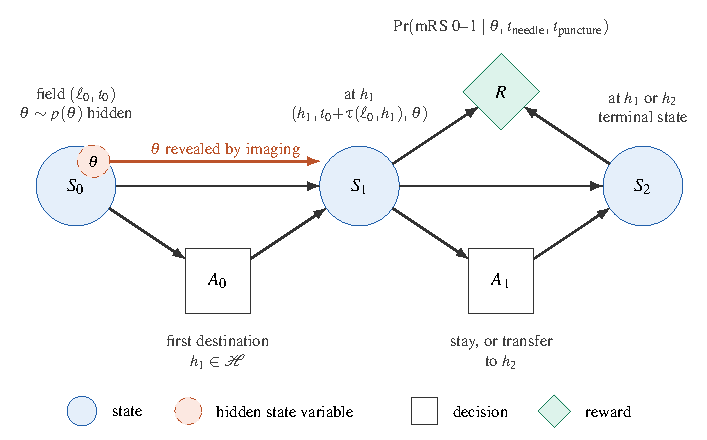
\includegraphics[width=0.9\textwidth]{fig_influence_standalone}
\caption{Influence diagram of the routing decision. The initial state $S_0$ holds the pickup location, the time since onset and the stroke subtype $\theta$, which is drawn from the population prior and hidden from the crew; the first decision $A_0$ observes location and time but not $\theta$. Arrival at $h_1$ advances the clock by the road travel time and imaging reveals $\theta$. The second decision $A_1$, made with $\theta$ known, is to treat at $h_1$ or transfer once to $h_2$. The reward is paid once, at the terminal state, as the probability of an excellent outcome given the subtype and the needle and puncture times the completed pathway implies (Table~\ref{tab:intervals}); the first leg earns no reward. For hemorrhage and stroke mimics the outcome does not depend on time.}
\label{fig:mdp}
\end{figure*}

\subsection{State space}
A state $s = (\ell, t, k, \sigma)$ comprises the patient's location $\ell$ (a pickup coordinate or a hospital), minutes since symptom onset $t$, whether the subtype is known $k \in \{\text{unknown}, \text{known}\}$, and the subtype $\sigma \in \{\text{LVO}, \text{nLVO}, \text{ICH}, \text{mimic}\}$. Pickup locations are sampled from high-resolution population density data~\cite{meta2019}, and onset-to-pickup time from 30 to 270 minutes, reflecting typical ranges to EMS contact~\cite{eddelien2021}. The subtype is drawn from the published prevalence of each category among patients with a positive prehospital LVO screen (Los Angeles Motor Scale $\geq 4$)~\cite{holodinsky2018}: $p_{\text{LVO}} = 0.454$, $p_{\text{nLVO}} = 0.109$, $p_{\text{ICH}} = 0.345$, $p_{\text{mimic}} = 0.092$. The planner never observes the drawn subtype while $k = \text{unknown}$; it reasons over the prior (Section~\ref{sec:method}). The subtype becomes known on arrival at any hospital, when imaging is assumed to occur.

\subsection{Action space}
Actions are discrete and location-dependent, and never route a patient to a lower capability tier. From the field, the patient may be transported to any hospital the road network reaches. From a non-stroke-center hospital the options are transfer to a thrombolysis-capable or EVT-capable center, or stay. From a thrombolysis-capable center, transfer to an EVT-capable center or stay. At an EVT-capable center the only action is to stay.

\subsection{Transition model}
A routing action moves the patient to the chosen hospital and advances the clock by the road travel time $\tau(\ell, \ell')$ obtained from the OpenRouteService routing engine on OpenStreetMap data; a transfer out of a hospital additionally incurs the door-in-door-out interval $T_{\text{DIDO}}$ before departure. On arrival the subtype becomes known. Transitions are deterministic given the action; all uncertainty enters through the subtype.

\subsection{In-hospital intervals}
Treatment is not instantaneous on arrival. We model three intervals, one value per interval for all hospitals of a tier, taken from national benchmarks (Table~\ref{tab:intervals}): door-to-needle $T_{\text{DTN}}$ for thrombolysis; door-to-puncture $T_{\text{DTP}}$ for EVT after direct arrival, and a shorter $T_{\text{DTP}}^{\text{tr}}$ for a transferred-in patient who arrives already imaged; and door-in-door-out $T_{\text{DIDO}}$ at the sending hospital. For a patient arriving directly at an EVT-capable center at onset time $t_a$, needle time is $t_a + T_{\text{DTN}}$ and puncture time $t_a + T_{\text{DTP}}$. At a thrombolysis-capable center, needle time is $t_a + T_{\text{DTN}}$ and, if the patient is transferred to an EVT-capable center at road time $\tau'$, puncture time is $t_a + T_{\text{DIDO}} + \tau' + T_{\text{DTP}}^{\text{tr}}$; which center, and whether to transfer at all, is the second decision. At a non-stroke-center hospital both treatments follow a transfer. Inter-facility transfers are not distance-limited; a pair is unreachable only if the road network has no route. For comparison, Holodinsky \emph{et al.}~\cite{holodinsky2018} assume door-to-needle 30, door-in-door-out 50 and door-to-puncture 60 (direct) or 30 (transfer) minutes in their base case, and 60 / 120 / 60--90 minutes in their slower scenarios; our base case lies between the two and is anchored to current registry medians and national targets.

\begin{table}[t]
\centering
\caption{In-hospital intervals in the base case (minutes) and the ranges examined in sensitivity analysis.}
\label{tab:intervals}
\resizebox{\columnwidth}{!}{\begin{tabular}{@{}lccl@{}}
\toprule
Interval & Base & Range & Source \\
\midrule
Door-to-needle $T_{\text{DTN}}$ & 45 & 30--60 & Target: Stroke III~\cite{targetstroke3} \\
Door-to-puncture, direct $T_{\text{DTP}}$ & 90 & 60--120 & Target: Stroke III~\cite{targetstroke3} \\
Door-to-puncture, transfer $T_{\text{DTP}}^{\text{tr}}$ & 60 & 45--90 & Target: Stroke III~\cite{targetstroke3} \\
Door-in-door-out $T_{\text{DIDO}}$ & 121 & 60--175 & GWTG-Stroke median, IQR 89--175~\cite{royan2026} \\
\bottomrule
\end{tabular}}
\end{table}


\subsection{Reward}
The reward is paid once, on the in-hospital decision that ends the episode, and is zero on the first leg. Its value is the probability of a good outcome, defined as an excellent outcome at 90 days (modified Rankin Scale 0--1), following Holodinsky \emph{et al.}~\cite{holodinsky2018}, evaluated at the needle and puncture times that the completed pathway implies: the first hospital $h_1$ reached at clock $t_1$, and the final hospital $h_2$ reached at $t_2$ ($h_2 = h_1$ if the patient stays). Thrombolysis is given at the first hospital on the pathway able to give it, so $t_n = t_1 + T_{\text{DTN}}$ if $h_1$ is thrombolysis- or EVT-capable and $t_n = t_2 + T_{\text{DTN}}$ if only $h_2$ is; thrombectomy requires an EVT-capable $h_2$, with $t_p = t_1 + T_{\text{DTP}}$ after direct arrival and $t_p = t_2 + T_{\text{DTP}}^{\text{tr}}$ after a transfer. For ischemic subtypes the outcome declines with onset-to-treatment time; for hemorrhage and mimics it is constant:
{\small\begin{align}
P_{\text{LVO,IVT}}(t_n) &= \max\{0.1328,\; 0.2359 - 4\!\times\!10^{-4} t_n + 2\!\times\!10^{-7} t_n^2\},\\
P_{\text{LVO,EVT}}(t_p) &= \max\{0.129,\; 0.3394 - 2\!\times\!10^{-4} t_p + 4\!\times\!10^{-8} t_p^2\},\\
P_{\text{LVO}} &= P_{\text{LVO,IVT}} + (1 - P_{\text{LVO,IVT}})\,P_{\text{LVO,EVT}},\\
P_{\text{nLVO}}(t_n) &= \max\{0.4622,\; 0.6343 - 5\!\times\!10^{-4} t_n - 5\!\times\!10^{-8} t_n^2\},\\
P_{\text{ICH}} &= 0.24, \qquad P_{\text{mimic}} = 0.90,
\end{align}}
where a treatment that the pathway does not provide contributes its untreated floor ($P_{\text{LVO,EVT}} = 0$ when no thrombectomy is performed), and $t_n, t_p \geq 270$ minutes yield the floor values. Because the reward is paid after imaging, it is always evaluated with the subtype known; subtype uncertainty enters only through the planner's expectation at the first decision (Section~\ref{sec:method}). Paying the reward once, rather than scoring each leg separately, is what makes the planner's objective and the reported outcome the same quantity.

% ---- IV. Solution Method. Budget 1.2 pages. Source: JAMA "Solution Approach" (1 para) and
% "Decision Tree Performance" (methods half). Expanded: forward search with marginalisation
% (NEW, from the May code change), decision-tree distillation as a first-class method (NEW).
\section{Solution Method}
\label{sec:method}

\subsection{Online planning by forward search}
\jama{JAMA "Solution Approach", expanded with the marginalisation step.}
We solve the MDP online with finite-horizon forward search~\cite{kochenderfer2022}: from the current state, every admissible action is expanded, its successor state evaluated, and the best action returned. A planning depth of two allows one inter-facility transfer after the initial destination, matching standard triage practice. \new{At the first step the subtype is unknown. Rather than recursing on a sampled subtype, which would let the planner peek at information the crew does not have, the value of a successor state is the prior-weighted sum over subtypes of the depth-one value from that state with the subtype known:
\begin{equation}
V_2(s) = \max_{a} \; \sum_{\sigma} p_\sigma \, \big[ R(s, a, s'_\sigma) + \max_{a'} R(s'_\sigma, a', s''_\sigma) \big],
\end{equation}
where $s'_\sigma$ is the arrival state with subtype $\sigma$ revealed. The action set at each hospital is small (transfer to one of the reachable higher-tier centres, or stay), so the search is exact.}

\new{[Add a short complexity paragraph: with $H$ hospitals the first step has at most $H$ actions and the second at most $H$ per subtype, so one decision costs $O(4H^2)$ reward evaluations, each of which needs at most two travel times; travel times from a pickup location to all hospitals are obtained in one matrix request to the routing engine and cached for the decision, and hospital-to-hospital times are cached across decisions. Measured latency is reported in Section~\ref{sec:results}.]}

\subsection{Comparator policies}
\jama{JAMA "Comparator Policies", moved here; tier names updated.}
We compare against three fixed rules. \emph{Nearest hospital} routes to the geographically closest hospital regardless of capability, the default where no triage protocol exists. \emph{Nearest EVT-capable centre} prefers the closest EVT-capable centre whenever one is reachable, as advocated in some states and implemented in Rhode Island; \new{if none is reachable it falls back to the nearest thrombolysis-capable centre, then to any hospital.} \emph{Nearest stroke centre} routes to whichever thrombolysis- or EVT-capable centre is closest, \new{with the same fallback.} \new{[Reviewer 2: note here that SF EMS policy is in effect "nearest stroke centre" and Santa Clara's is "nearest EVT-capable centre for LAMS-positive patients", so the heuristics are not straw men; cite the policies.]}

\subsection{Distilling the policy into a decision tree}
\jama{JAMA "Decision Tree Performance" first paragraph, methods part.}
For use by EMS crews without computation, we approximate the MDP policy with a decision tree. Each simulated patient is labelled with the MDP's recommended destination, translated into a tier (EVT-capable, thrombolysis-capable, non-stroke-centre). Features are time since onset, road travel time to the nearest hospital of each tier, reachability indicators, and the pairwise differences and ratios of those travel times. \new{Trees of depth 1 to 10 and an unconstrained tree are trained on \pending{n} labelled patients and evaluated on \pending{n} held-out patients never used for training, scoring each tree's recommended destination with the same reward model and comparing it with the MDP's recommendation for the same patient. We report, per depth, the mean outcome, the mean loss relative to the MDP, the share of the MDP's gain over nearest-hospital routing that the tree recovers, and the number of leaves, and select the shallowest tree within 1\% of the MDP. The tree is a static artefact: it can be printed, embedded in a dispatch system, or read aloud, and it changes only when the hospital table or the travel-time engine does.}

% ---- V. Experimental Setup. Budget 1.2 pages. Source: JAMA "Study Design", "Simulation Model
% Overview", "Action Space" (hospital verification sentence). Mostly NEW detail the reviewers
% asked for: cohort characteristics, replicates, hospital verification, sensitivity design.
\section{Experimental Setup}
\label{sec:setup}

\subsection{Regions and hospital networks}
\jama{JAMA "Study Design and Setting" + hospital-verification sentence, updated to the 2 Oct 2026 verification.}
We evaluate two regions with different network structures and stroke-system policies: the nine-county San Francisco Bay Area, California, a decentralised system with \pending{11} EVT-capable centres, \pending{44} thrombolysis-capable centres and \pending{6} non-stroke-centre hospitals (\pending{61} in total), and the state of Rhode Island, a centralised system with one EVT-capable centre, eight thrombolysis-capable centres and no uncertified acute-care hospital. \new{Hospital designations were verified on 2 October 2026 against county EMS agency receiving-facility lists, the Rhode Island Department of Health stroke designation list, certifying-body records and hospital system pages; coordinates were checked against street addresses. Four Bay Area hospitals perform thrombectomy without Comprehensive or Thrombectomy-Capable certification; they are thrombolysis-capable in the primary analysis and EVT-capable in a sensitivity analysis. Designations change (two Bay Area hospitals changed in 2026), so the hospital table is an input to the method rather than part of it.} \new{[Add one sentence on EMS context: SF routes to the closest stroke centre without LVO tiering; Santa Clara routes LAMS-positive patients to the closest EVT-capable centre; Marin transfers LVO patients out of county, often by air. Cite policies.]}

\subsection{Simulated cohorts}
\jama{JAMA "Simulation Model Overview", with replicate detail added (Reviewer 2: how many simulations, what characteristics).}
Each replicate samples 1,000 pickup locations without replacement from a population-weighted pool of 10,000 points~\cite{meta2019}, draws onset-to-pickup time uniformly on 30--270 minutes and the subtype from the LAMS-positive prior, and routes every patient under each policy. \new{We run 10 replicates per region with distinct seeds, giving 10,000 patient-policy pairs per policy and between-replicate confidence intervals. The same patients are routed under every policy, so comparisons are paired. A patient is excluded only if no policy can reach a hospital within the catchment radius (\pending{k} of 10,000).} \new{[Reviewer 1 asked about the grid: state here that the 200$\times$200 grid with 5 patients per cell is the visualisation layer for the geographic analysis, not the cohort used for the main results.]}

\subsection{Travel times and catchment}
\new{Travel times are computed on the OpenStreetMap road network with OpenRouteService~8.0 (driving-car profile) hosted locally. Candidate destinations for the initial transport are restricted to facilities within 80~km of the pickup location, an EMS catchment assumption; inter-facility transfers are computed by road for all pairs without a distance restriction. Travel times are deterministic in the planner; sensitivity to travel-time error is assessed post hoc (below).}

\subsection{Outcome measures and statistics}
\new{The primary measure is the probability of an excellent 90-day outcome (mRS 0--1) per patient. For each pair of policies we report the mean paired difference with a 95\% confidence interval across the 10 replicates ($t_9$), the paired $t$-test with Bonferroni correction for the five comparisons, and Cohen's $d_z$. We distinguish the \emph{planning} reward (the prior-weighted mixture the planner optimises) from the \emph{realised} reward (the subtype-specific outcome given the drawn subtype); tables report realised rewards unless stated. Equity is assessed by stratifying paired differences by census-tract median household income quartile and RUCA urbanicity, for the MDP against nearest-hospital and against both heuristics.}

\subsection{Sensitivity analyses}
\new{(i) Travel-time error: multiplicative log-normal noise ($\sigma = 0.10, 0.20$) and systematic bias ($\times 0.70$ to $\times 1.30$) applied to the recorded first-leg travel time, with one draw per patient-destination so identical routes receive identical perturbations; rewards are recomputed and the paired comparisons repeated. (ii) In-hospital intervals: $T_{\text{DIDO}} \in \{60, 90, 121, 175\}$ minutes, rewards recomputed post hoc for the policies as planned under the base case. (iii) EVT definition: the four uncertified thrombectomy sites treated as EVT-capable, with the policy re-planned. (iv) Decision-tree depth: 1 to 10 and unconstrained.}

\subsection{Latency}
\new{Per-decision wall-clock time of the planner is measured on \pending{machine spec} for 50 patients at planning depths 1 to 4, with the routing engine on the same machine, after warm-up. We report mean, median, 95th and 99th percentiles.}

\new{[Reproducibility sentence: all randomness seeded; pinned Julia environment; code and hospital tables released on acceptance.]}

% ---- VI. Results. Budget 2.3 pages: ~900 words + Table II (main), Table III (sensitivity),
% Table IV (tree sweep + latency), Fig. 1 (histogram or paired-difference plot), Fig. 2 (maps),
% Fig. 3 (tree). JAMA results text is kept as the narrative frame; EVERY number is pending.
\section{Results}
\label{sec:results}

\subsection{Primary comparison: San Francisco Bay Area}
\jama{JAMA "Simulation Outcomes: Bay Area", structure kept; numbers were single-run and are replaced.}
Across 10 replicates of 1,000 patients, the MDP policy raised the mean probability of a good outcome from \pending{0.xxx} under nearest-hospital routing to \pending{0.xxx} (paired difference \pending{0.0xx}, 95\% CI \pending{a--b}, $d_z$ = \pending{x.x}; Table~\ref{tab:main}). The median rose from \pending{0.xxx} to \pending{0.xxx}. \jama{Keep the "spike at the floor value" explanation if the histogram still shows it.} A spike in the outcome distribution at \pending{0.xxx} reflects patients who reached treatment outside the window in which earlier arrival adds benefit; for them routing cannot help, which bounds the achievable gain of any policy.

Against the heuristics, nearest-hospital routing underperformed all alternatives. The MDP policy outperformed the nearest-stroke-centre rule by \pending{0.0xx} (95\% CI \pending{a--b}) and the nearest-EVT-centre rule by \pending{0.0xx} (95\% CI \pending{a--b}). \jama{JAMA operational-burden paragraph, numbers pending.} Where the MDP and nearest-EVT-centre policies diverged (\pending{n} of 10,000 cases), \pending{m} had identical predicted outcomes, yet the nearest-EVT-centre rule added a mean \pending{x.x} minutes of transport, and it concentrated transports on \pending{k} hospitals against \pending{j} under the MDP. The reward does not penalise travel that leaves the outcome unchanged, so it understates the operational cost of fixed bypass rules.

\begin{table}[t]
\centering
\caption{Bay Area, 10 replicates $\times$ 1,000 patients. Probability of an excellent outcome (mRS 0--1 at 90 days), realised reward. Paired differences with 95\% CI across replicates.}
\label{tab:main}
\begin{tabular}{@{}lccc@{}}
\toprule
Policy & Mean & Median & Hospitals used \\
\midrule
MDP (depth 2) & \pending{} & \pending{} & \pending{} \\
Nearest hospital & \pending{} & \pending{} & \pending{} \\
Nearest EVT-capable centre & \pending{} & \pending{} & \pending{} \\
Nearest stroke centre & \pending{} & \pending{} & \pending{} \\
Decision tree (depth \pending{d}) & \pending{} & \pending{} & \pending{} \\
\midrule
\multicolumn{4}{@{}l}{Paired difference, mean (95\% CI), Bonferroni-adjusted $p$} \\
MDP $-$ Nearest hospital & \multicolumn{3}{l}{\pending{}} \\
MDP $-$ Nearest EVT-capable & \multicolumn{3}{l}{\pending{}} \\
MDP $-$ Nearest stroke centre & \multicolumn{3}{l}{\pending{}} \\
\bottomrule
\end{tabular}
\end{table}

\subsection{Geographic and equity analysis}
\jama{JAMA "Geographic Analysis of Outcomes": the "71\%" now comes from CA\_grid\_hotspot\_summary.csv (relative improvement per cell); the equity claim is now vs heuristics as well (Reviewer 2).}
To locate where routing matters most, we simulated five patients in each cell of a 200$\times$200 grid over the Bay Area and mapped the mean outcome under each policy (Fig.~\ref{fig:maps}). Relative to nearest-hospital routing, the MDP improved the cell mean by a median of \pending{x}\% and by more than \pending{25}\% in \pending{n} cells, with a maximum of \pending{xx}\%; no cell worsened by more than \pending{x}. \jama{Keep the Livermore/Hayward/Fremont vs SF/Palo Alto/San Jose contrast if it survives the reruns.} The largest gains were in \pending{communities}, which lie farther from EVT-capable centres; San Francisco, Palo Alto and San Jose, with proximate EVT-capable centres, changed little. Stratified by tract income quartile and urbanicity (Table~\ref{tab:equity}), the MDP's gain over nearest-hospital routing was \pending{largest / similar} in the lowest income quartile and in rural tracts; against the nearest-EVT-centre heuristic the gain was \pending{x}, showing that \pending{the equity benefit is / is not} specific to the MDP rather than to any bypass rule.

\begin{table}[t]
\centering
\caption{Paired difference in probability of a good outcome by stratum (mean, 95\% CI). Rural stratum is small (\pending{n} tracts).}
\label{tab:equity}
\begin{tabular}{@{}lccc@{}}
\toprule
Stratum & MDP $-$ Nearest & MDP $-$ Nearest EVT & MDP $-$ Nearest SC \\
\midrule
Income Q1 (lowest) & \pending{} & \pending{} & \pending{} \\
Income Q2 & \pending{} & \pending{} & \pending{} \\
Income Q3 & \pending{} & \pending{} & \pending{} \\
Income Q4 & \pending{} & \pending{} & \pending{} \\
Urban & \pending{} & \pending{} & \pending{} \\
Rural & \pending{} & \pending{} & \pending{} \\
\bottomrule
\end{tabular}
\end{table}

\begin{figure}[t]
\centering
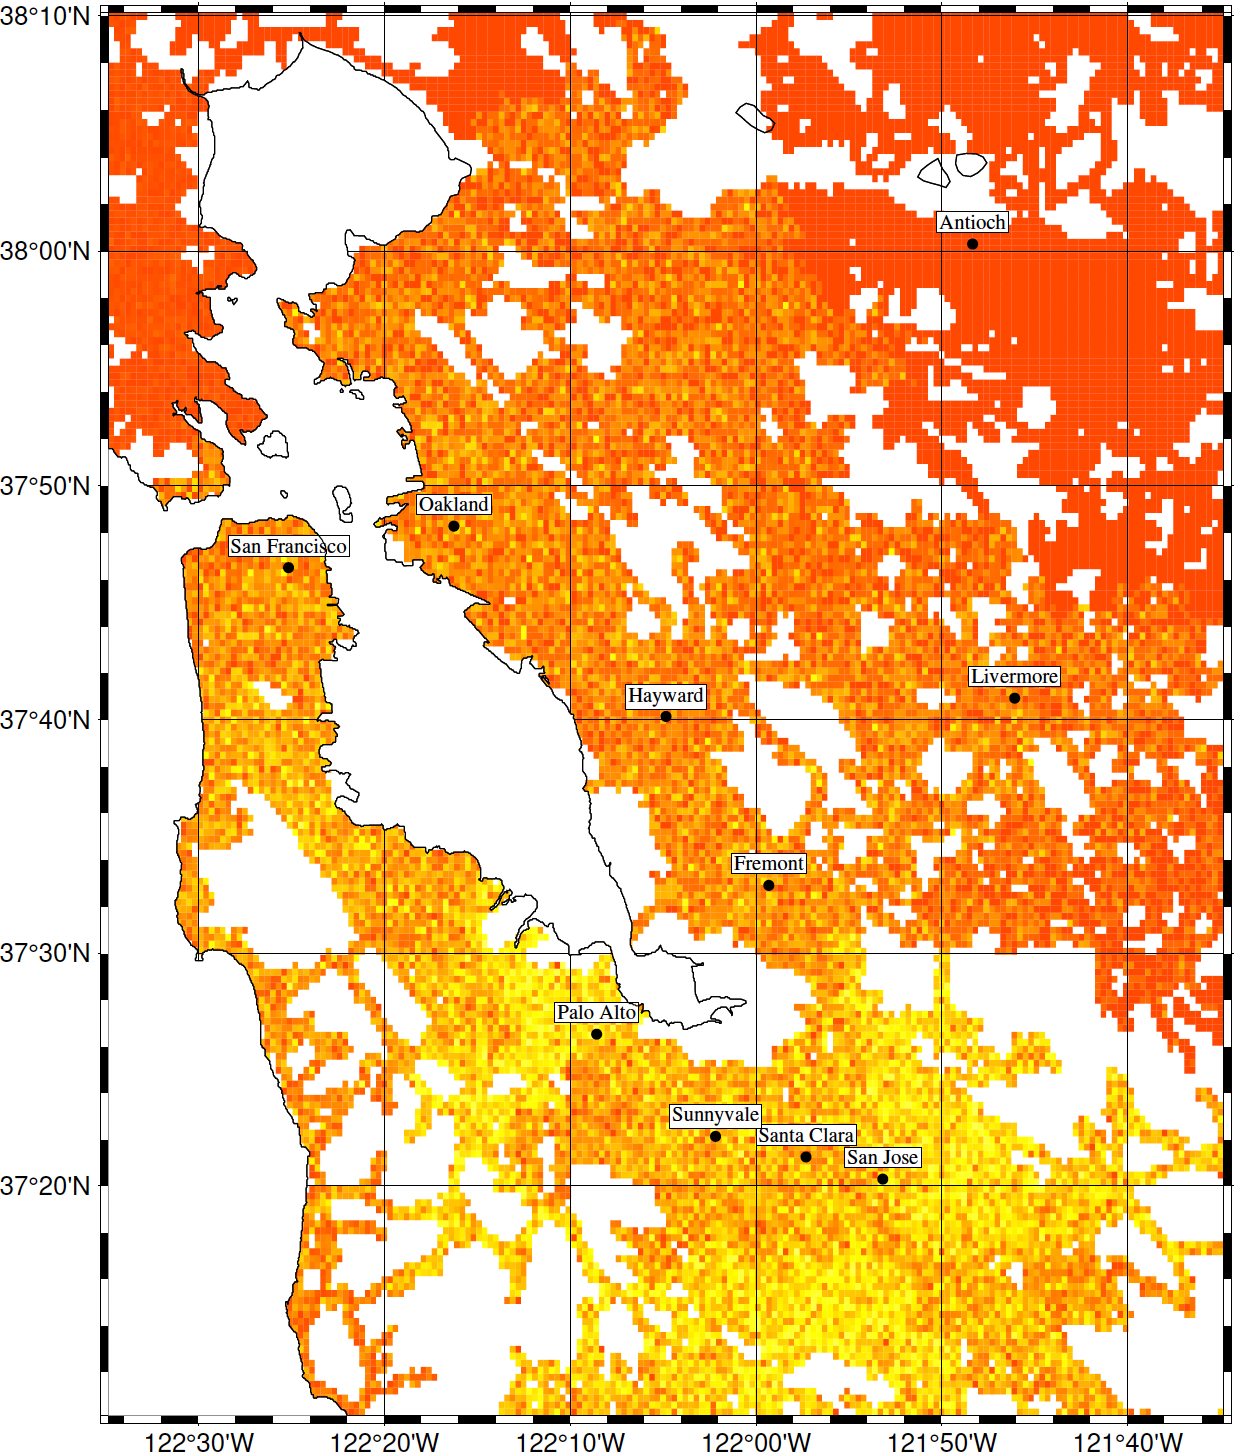
\includegraphics[width=0.49\columnwidth]{jama_fig2a_nearest_map}\hfill
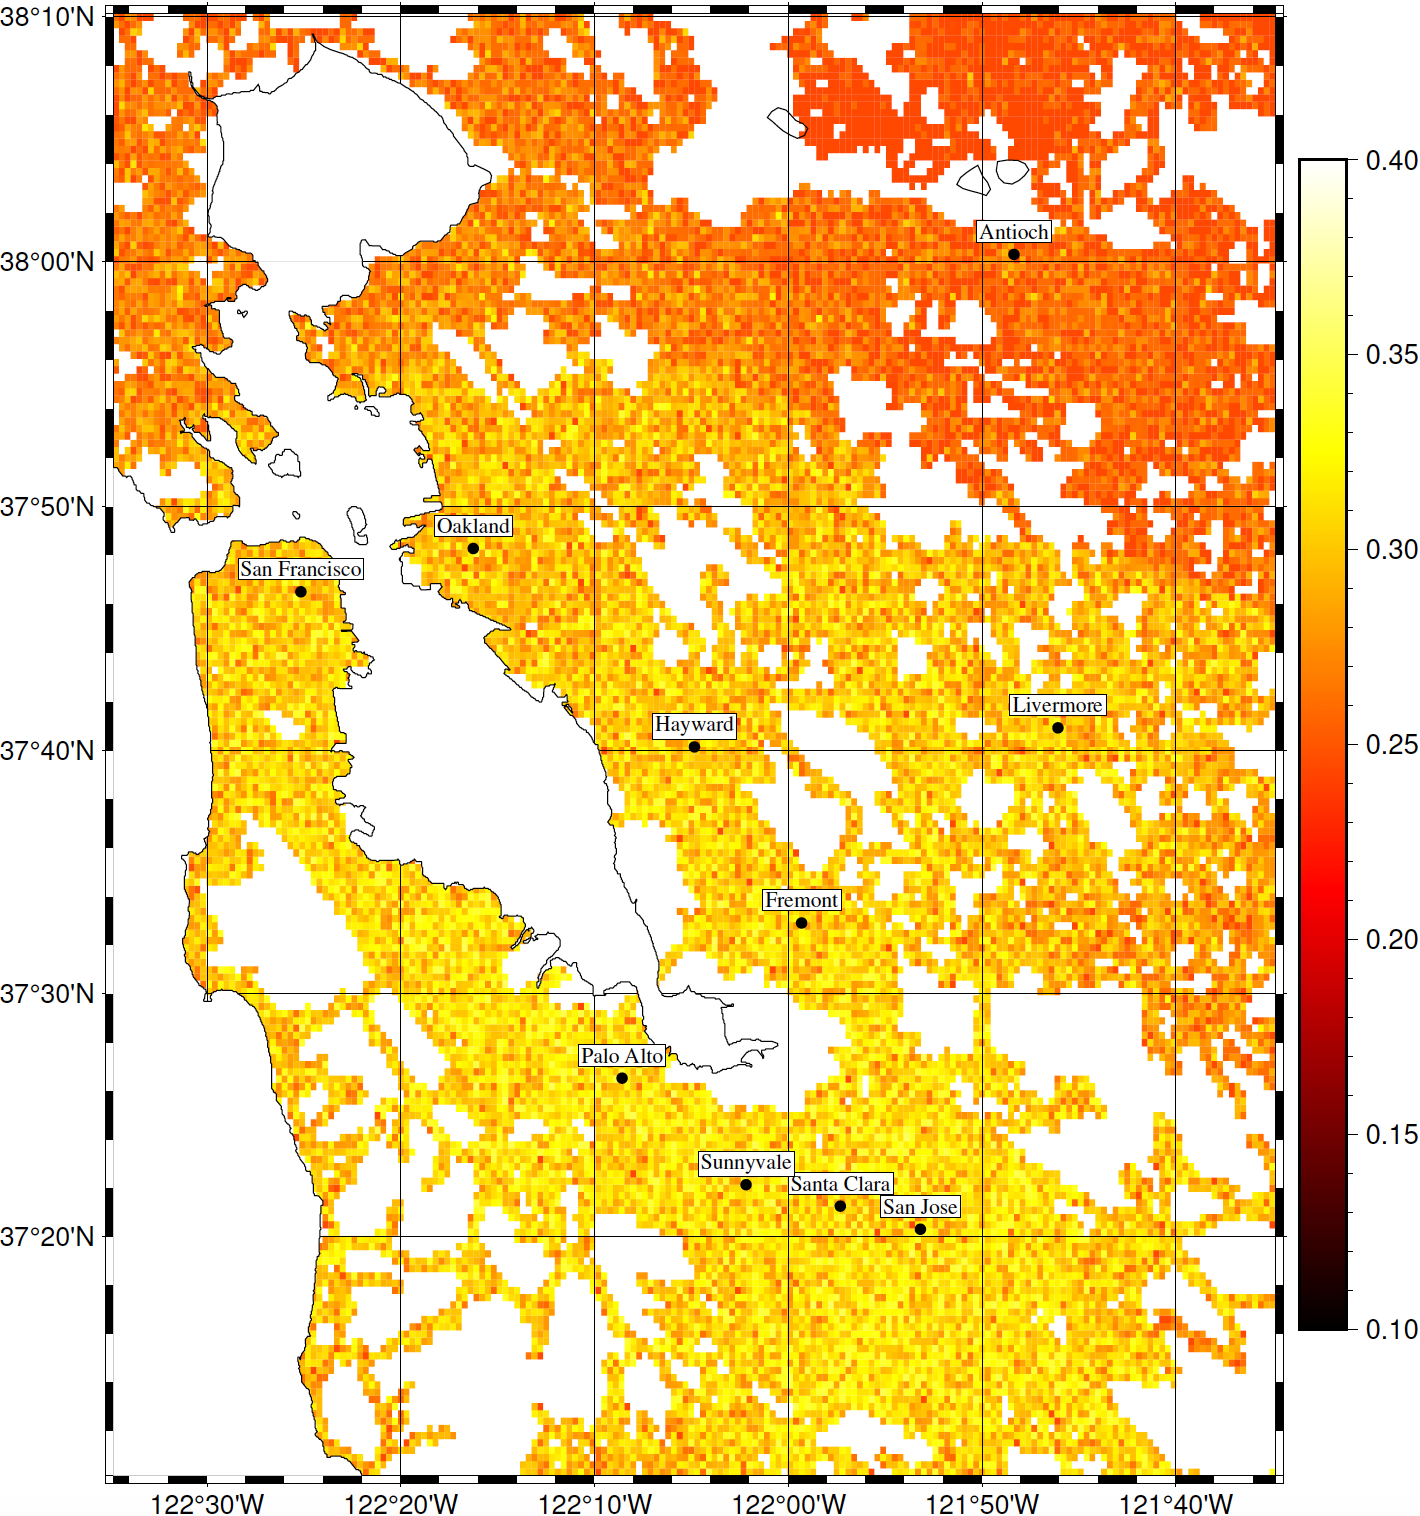
\includegraphics[width=0.49\columnwidth]{jama_fig2b_optimal_map}\\[2pt]
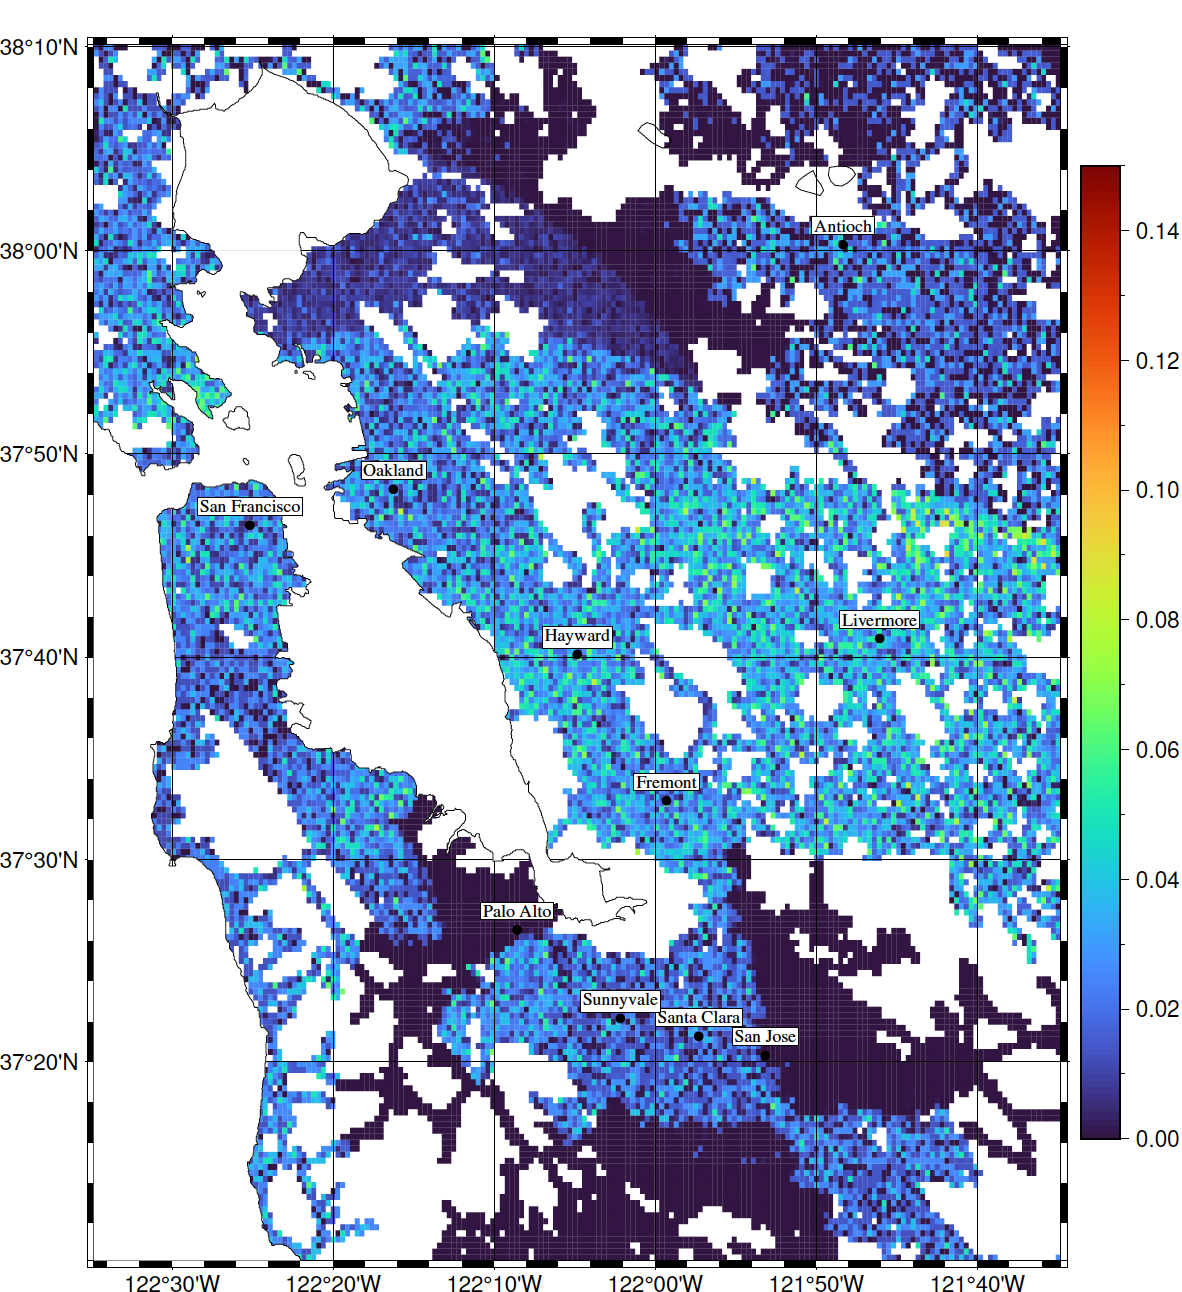
\includegraphics[width=0.7\columnwidth]{jama_fig3_difference_map}
\caption{\pending{Regenerate from CA\_grid\_cell\_means.csv.} Mean probability of a good outcome per grid cell under nearest-hospital routing (top left) and the MDP policy (top right), and their difference (bottom). Warmer colours indicate higher values.}
\label{fig:maps}
\end{figure}

\subsection{Sensitivity analyses}
\new{Table~\ref{tab:sens} reports the MDP-minus-nearest difference under perturbed travel times and alternative in-hospital intervals. [Narrative to write once numbers exist. Expected: the difference is stable under $\pm 20\%$ noise and $\times 0.7$--$1.3$ bias; it grows with $T_{\text{DIDO}}$, because longer door-in-door-out penalises drip-and-ship and favours direct transport to EVT-capable centres, consistent with the registry association between DIDO and outcome~\cite{royan2026}. Under the on-site EVT definition (15 EVT-capable centres) the difference is \pending{x}.]}

\begin{table}[t]
\centering
\caption{Sensitivity of the MDP $-$ nearest-hospital difference (mean, 95\% CI across replicates).}
\label{tab:sens}
\begin{tabular}{@{}llc@{}}
\toprule
Analysis & Setting & Difference \\
\midrule
Base case & & \pending{} \\
Travel-time noise & $\sigma = 0.10$ / $0.20$ & \pending{} / \pending{} \\
Travel-time bias & $\times 0.70$ / $0.90$ / $1.10$ / $1.30$ & \pending{} \\
Door-in-door-out & 60 / 90 / 175 min & \pending{} \\
EVT definition & on-site (15 centres) & \pending{} \\
\bottomrule
\end{tabular}
\end{table}

\subsection{Decision-tree policy}
\jama{JAMA "Decision Tree Performance", evaluation half; depth is now chosen by the sweep.}
Fig.~\ref{fig:tree} shows the selected tree. On \pending{n} held-out patients it achieved a mean outcome of \pending{0.xxx} against \pending{0.xxx} for the MDP, recovering \pending{xx}\% of the MDP's gain over nearest-hospital routing with \pending{k} leaves (Table~\ref{tab:tree}). Shallower trees lose \pending{...}; deeper trees add leaves without material gain. \new{[One sentence on which splits dominate: time since onset and the EVT-centre travel-time margin.]}

\begin{table}[t]
\centering
\caption{Decision-tree depth sweep on held-out patients, and planner latency per decision.}
\label{tab:tree}
\begin{tabular}{@{}lcccc@{}}
\toprule
Depth & Leaves & Mean outcome & Gain recovered & \\
\midrule
1 / 2 / 3 / 4 & \pending{} & \pending{} & \pending{} & \\
5 / 6 / 8 / 10 / $\infty$ & \pending{} & \pending{} & \pending{} & \\
\midrule
Planning depth & Median (ms) & p95 (ms) & p99 (ms) & \\
1 / 2 / 3 / 4 & \pending{} & \pending{} & \pending{} & \\
\bottomrule
\end{tabular}
\end{table}

\begin{figure}[t]
\centering
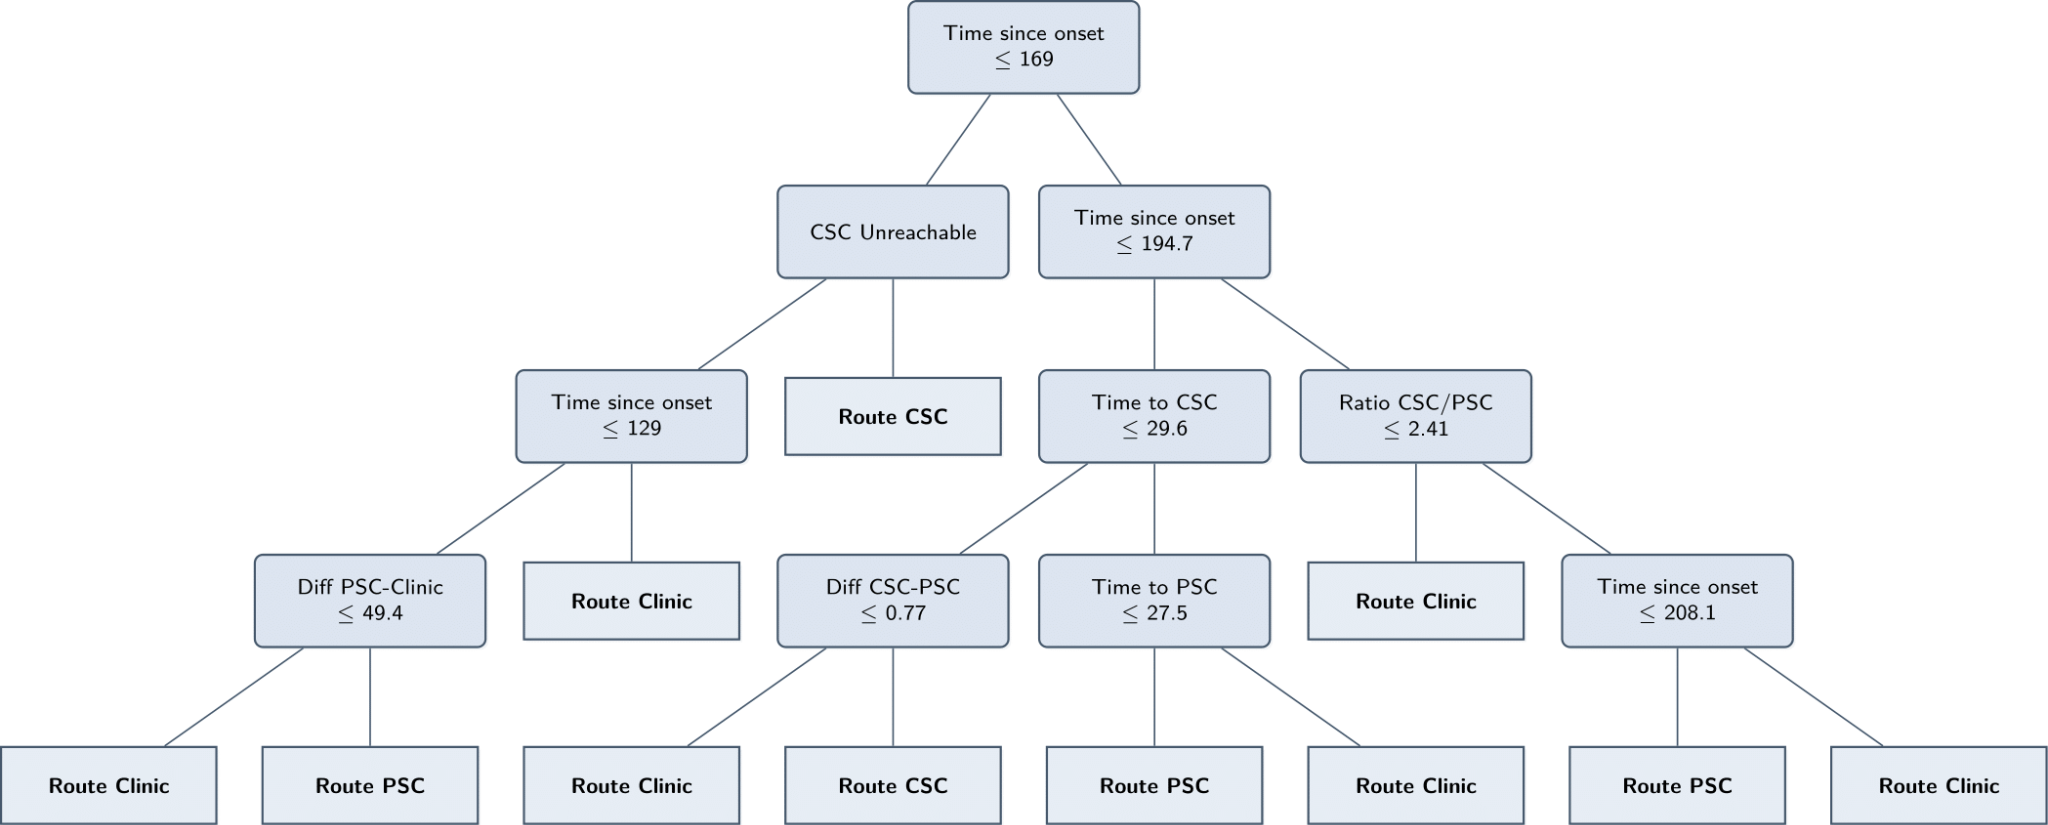
\includegraphics[width=\columnwidth]{jama_fig4_decision_tree}
\caption{\pending{Regenerate for the selected depth.} Decision-tree approximation of the MDP policy. Left and right branches are ``no'' and ``yes''.}
\label{fig:tree}
\end{figure}

\subsection{Real-time feasibility}
\new{A depth-2 decision took a median of \pending{xxx}~ms (p95 \pending{xxx}~ms) on \pending{hardware}, within any dispatch window; depth 3 and 4 cost \pending{x} and \pending{y}~s, which with the negligible outcome gain beyond depth 2 (\pending{...}) justifies the chosen depth. The decision tree needs no computation at all.}

\subsection{Rhode Island}
\jama{JAMA "Simulation Outcomes: Rhode Island"; now all comparisons, 10 replicates (Reviewer 2).}
In Rhode Island the MDP and the state's nearest-EVT-centre protocol gave nearly identical mean outcomes (\pending{0.xxx} vs \pending{0.xxx}; difference \pending{0.00x}, 95\% CI \pending{a--b}), while the MDP routed to \pending{k} hospitals against one, and both outperformed nearest-hospital and nearest-stroke-centre routing by \pending{x} and \pending{y} (Table~\ref{tab:ri}). \new{[Interpretation: in a small state with one EVT centre the optimal policy largely coincides with the centralised protocol, and the value of the MDP is in load distribution rather than outcome.]}

\begin{table}[t]
\centering
\caption{Rhode Island, 10 replicates $\times$ 1,000 patients.}
\label{tab:ri}
\begin{tabular}{@{}lccc@{}}
\toprule
Policy & Mean & Median & Hospitals used \\
\midrule
MDP (depth 2) & \pending{} & \pending{} & \pending{} \\
Nearest hospital & \pending{} & \pending{} & \pending{} \\
Nearest EVT-capable centre & \pending{} & \pending{} & 1 \\
Nearest stroke centre & \pending{} & \pending{} & \pending{} \\
\bottomrule
\end{tabular}
\end{table}

% ---- VII. Discussion. Source: JAMA Discussion paragraphs 1 and 2; limitations are new, one
% per JAMA reviewer objection. The Regional Medical Center aside is dropped.
\section{Discussion}
\label{sec:discussion}

The MDP policy improves expected outcomes over nearest-hospital routing in a decentralized system and matches the centralized protocol of a small state while spreading load across hospitals. By accounting for hospital capability, elapsed time and the cost of a later transfer, it delivers more effective routing where it matters for equity: in areas distant from EVT-capable centers, with no systematic loss in well-served areas, and the stratified analysis shows the gain over the bypass heuristics as well as over the default. The decision tree carries this benefit into a form a crew can apply, and a decision costs milliseconds.

Two practical considerations merit attention. The MDP increases mean initial transport time to 16.7 minutes from 9.4 under nearest-hospital routing in the Bay Area, but it reduces downstream transfers and their delays; for LVO patients, bypassing a closer but less capable hospital means arriving at an EVT-capable center within the therapeutic window. At the same time the MDP travels less than the nearest-EVT-center rule (21.4 minutes), because it declines the detour for patients whose outcome it cannot change. The second consideration is hospital load, discussed below.

The in-hospital intervals matter as much as the road network. With door-in-door-out at 60 minutes the gain over nearest-hospital routing is a third of its value at the registry median, and at the registry upper quartile it is larger still: the value of intelligent routing grows with the inefficiency of transfer. Agencies with fast transfer pathways should expect smaller gains, and an agency that measures its own intervals can substitute them directly.

\subsection{Limitations}
\emph{Capacity and queueing.} The model assumes every hospital can accept every patient routed to it. We do not model bed or angiography-suite availability, diversion, or interaction between concurrent patients. The load-distribution result (the MDP uses 51 hospitals where the nearest-EVT rule uses 10, and places 35\% rather than 52\% of patients at the two busiest centers) is a qualitative indication that the policy does not concentrate demand, not a capacity analysis. A capacity-aware extension would add hospital state to the MDP and is the main direction for future work.

\emph{Validation against observed outcomes.} Results are simulated. The outcome model is taken from published onset-to-treatment curves~\cite{holodinsky2018}, travel times from a routing engine, and in-hospital intervals from national registries; the composition has not been validated against a cohort with observed routing and outcomes. The sensitivity analyses bound the effect of the main inputs but do not substitute for validation, which requires EMS and hospital record linkage.

\emph{In-hospital intervals.} One value per interval for all hospitals of a tier. Real door-to-needle, door-to-puncture and door-in-door-out times vary widely between hospitals and over time; the DIDO sensitivity shows the direction and size of the effect, and hospital-specific intervals can be substituted where an agency has them.

\emph{Patient population.} The cohort is LAMS~$\geq$~4 with onset within 270 minutes. Prehospital scales identify LVO imperfectly, and EVT benefit extends to 24 hours for selected patients. The outcome curves used here are defined to 270 minutes; extending the model to the late window needs late-window outcome functions and is left for future work. Less severe strokes also face routing decisions that the present scope does not address.

\emph{Hemorrhage.} The outcome for intracerebral hemorrhage is time-invariant in the reward. Evidence that timely bundled care improves ICH outcomes~\cite{interact3} suggests a time-dependent function would be appropriate when one is available; its absence biases the model against any destination choice motivated by ICH, which is conservative for the MDP's gains.

\emph{Capability definitions.} Hospitals are classified by verified certification. Some hospitals perform thrombectomy without certification; the on-site sensitivity analysis treats them as EVT-capable and does not change the conclusions. Designations change over time; the method takes the table as input.

\emph{Generalizability and the baseline.} Both regions are dense relative to much of the United States, and routing protocols vary by jurisdiction. Nearest-hospital routing is a lower bound on current practice rather than a description of it everywhere; the heuristic comparators correspond to the protocols actually in use, which is why both are reported. Air transport is not modeled.

\emph{Travel times.} Deterministic routing-engine estimates stand in for traffic-dependent times; the noise and bias analyses cover the plausible range of error but not time-of-day structure.

\subsection{Deployment path and other applications}
The deployable artifact is the decision tree, re-derived whenever the hospital table changes, with the MDP as the reference it is checked against. The natural next step is a prospective evaluation with an EMS agency in which the tree's recommendation is recorded alongside the crew's destination and the patient's eventual outcome. The formulation is not specific to stroke: any time-critical dispatch decision with tiered receiving facilities, an unobserved patient class revealed on arrival, and a possible secondary transfer (trauma, ST-elevation myocardial infarction, aortic dissection) has the same structure and would need only its own outcome curves and facility table.

% ---- VIII. Conclusion. Rewritten from the JAMA conclusion; claims limited to what the results show.
\section{Conclusion}
We formulated prehospital stroke routing as an MDP over patient location, time since onset and subtype uncertainty, with capability-classified hospitals, road travel times, inter-facility transfer and published in-hospital intervals, and solved it online in milliseconds. In simulation across two regions the policy raised the expected probability of an excellent outcome over nearest-hospital routing by 0.02 on a base of 0.36, matched a centralized bypass protocol while sparing unnecessary detours and distributing load, and was robust to travel-time error and to the definition of EVT capability, with a gain that grows with door-in-door-out time. A one-split decision tree recovered 99.4\% of the gain and requires no computation to apply. The hospital table and routing engine are inputs, so the approach transfers to other regions by changing data. Capacity modeling and validation against observed outcomes are the next steps before deployment.


\ifanon\else
\section*{Acknowledgments}
\jama{From JAMA, unchanged.}
We thank Dr.~Mahesh V. Jayaraman for his expert guidance in understanding the medical landscape and the implementation of Rhode Island's stroke routing policy, Zara Rutherford for her contributions to a mobile application prototype for EMS use, and Dr.~Sophie Ostmeier for her guidance throughout this project.
\fi

\bibliographystyle{IEEEtran}
\bibliography{refs}

\end{document}
